\subsection{Performance}

\subsubsection{SimCLR}

\paragraph{Nearest neighbors in image space}
The nearest neighbors are calculated in feature space after which the ten corresponding nearest neighbors of a random tile are shown.
The nearest neighbors are calculated for a SimCLR pretrained backbone as well as a backbone pretrained on ImageNet.
The results are shown in \cref{fig:nearest-neighbours-image-space}.

\begin{figure*}
    \centering
    \begin{tabular}[\linewidth]{rc}
        \raisebox{1.6\normalbaselineskip}[0pt][0pt]{\rotatebox[origin=c]{90}{\tiny ImageNet}} & 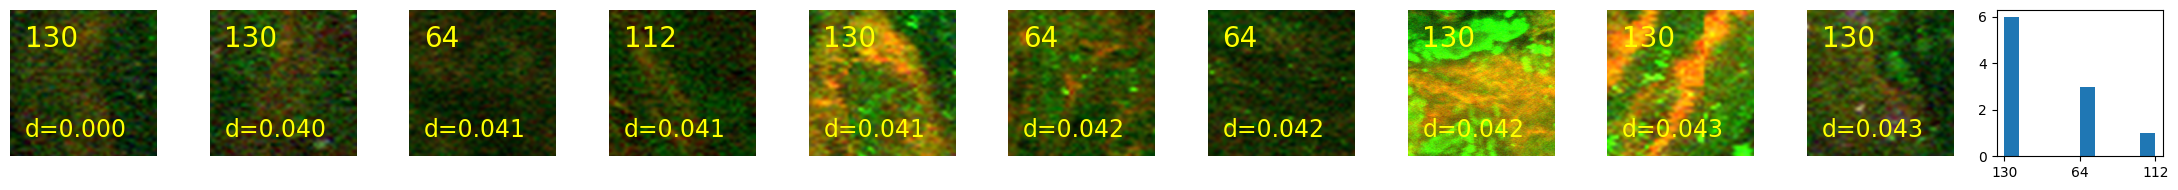
\includegraphics[width=\linewidth]{pediatric-brain-tumours/images/imagenet-nn-1.png} \\
        \raisebox{1.6\normalbaselineskip}[0pt][0pt]{\rotatebox[origin=c]{90}{\tiny SimCLR}} & 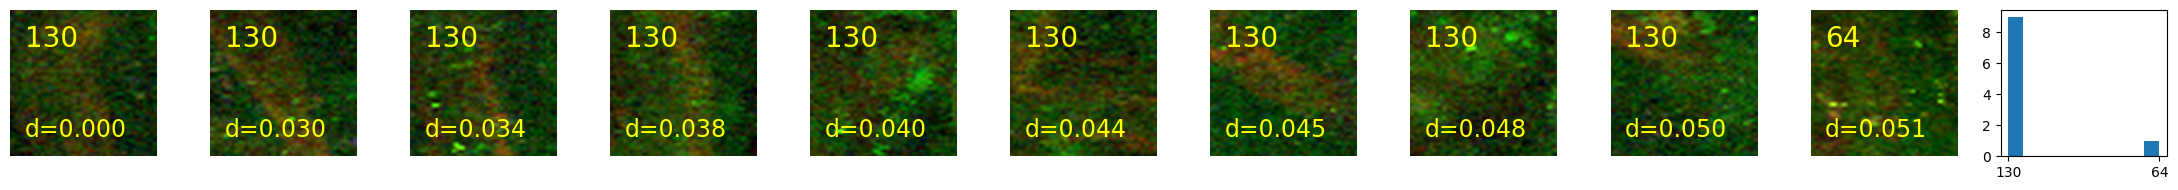
\includegraphics[width=\linewidth]{pediatric-brain-tumours/images/simclr-nn-1.png} \\
        \midrule
        \raisebox{1.6\normalbaselineskip}[0pt][0pt]{\rotatebox[origin=c]{90}{\tiny ImageNet}} & 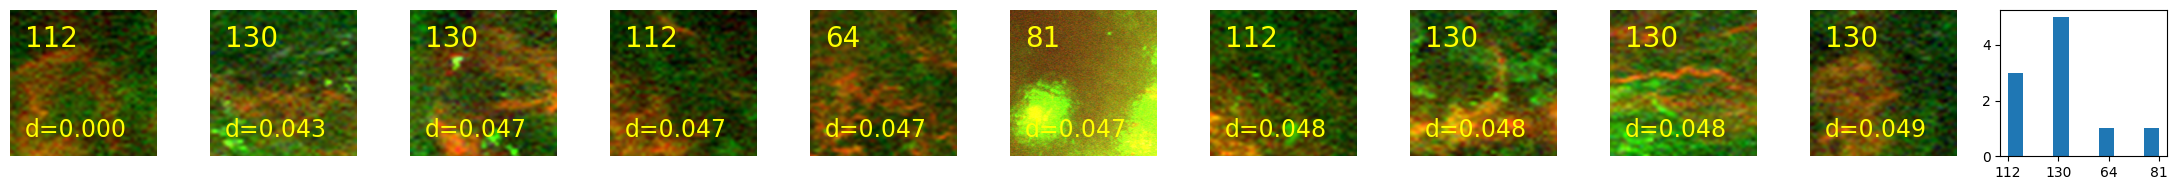
\includegraphics[width=\linewidth]{pediatric-brain-tumours/images/imagenet-nn-2.png} \\
        \raisebox{1.6\normalbaselineskip}[0pt][0pt]{\rotatebox[origin=c]{90}{\tiny SimCLR}} & 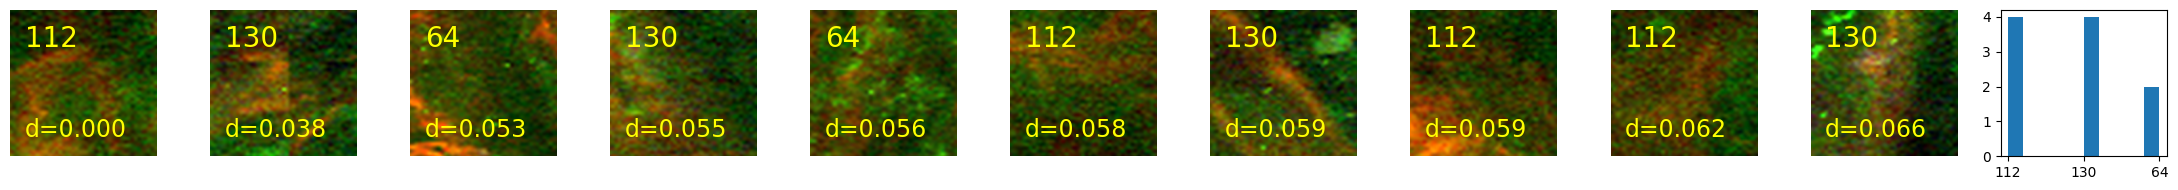
\includegraphics[width=\linewidth]{pediatric-brain-tumours/images/simclr-nn-2.png} \\
        \midrule
        \raisebox{1.6\normalbaselineskip}[0pt][0pt]{\rotatebox[origin=c]{90}{\tiny ImageNet}} & 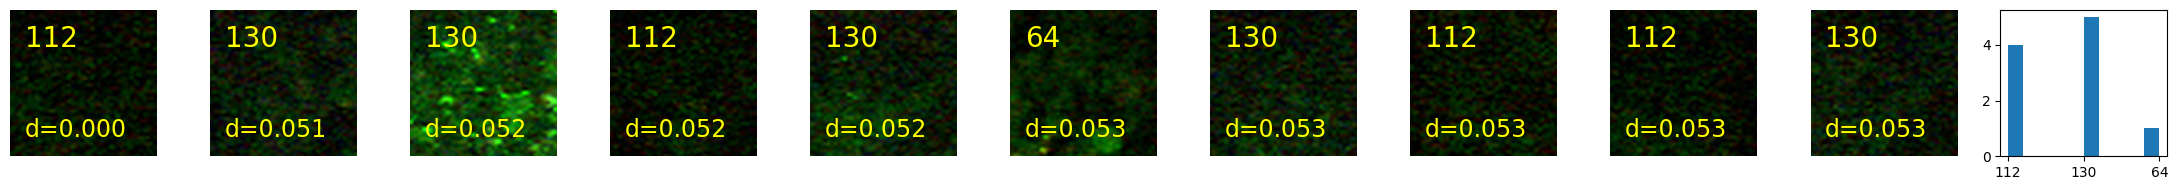
\includegraphics[width=\linewidth]{pediatric-brain-tumours/images/imagenet-nn-3.png} \\
        \raisebox{1.6\normalbaselineskip}[0pt][0pt]{\rotatebox[origin=c]{90}{\tiny SimCLR}} & 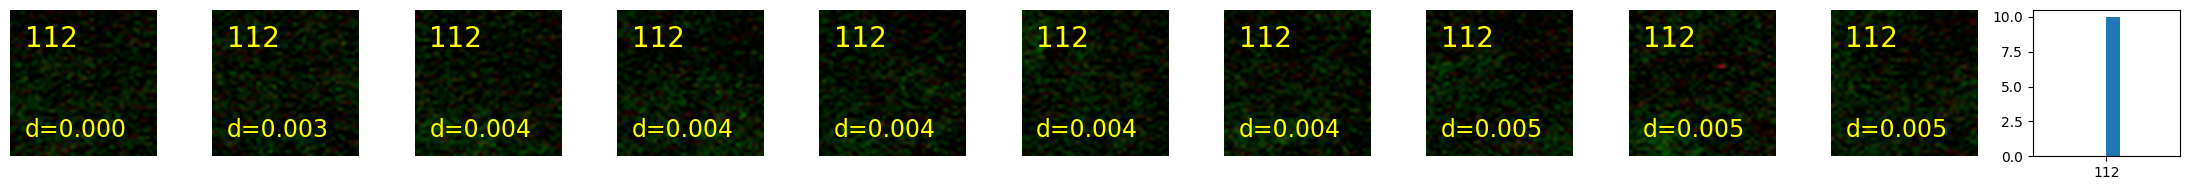
\includegraphics[width=\linewidth]{pediatric-brain-tumours/images/simclr-nn-3.png} \\
        \midrule
        \raisebox{1.6\normalbaselineskip}[0pt][0pt]{\rotatebox[origin=c]{90}{\tiny ImageNet}} & 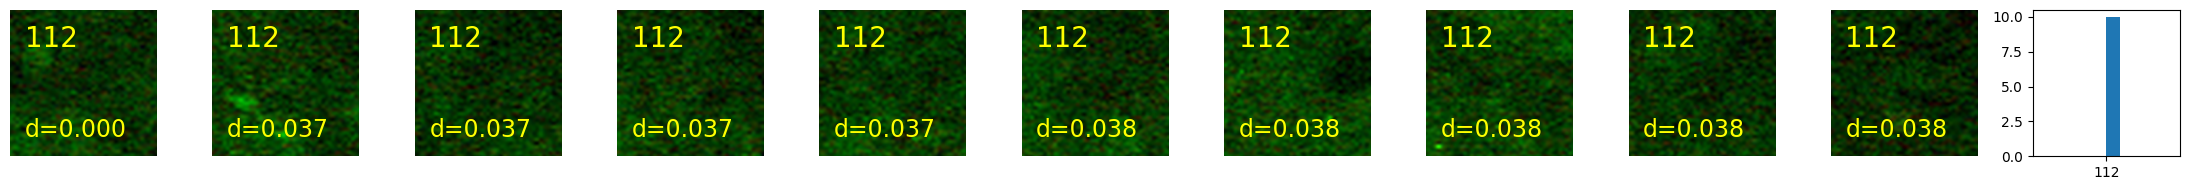
\includegraphics[width=\linewidth]{pediatric-brain-tumours/images/imagenet-nn-5.png} \\
        \raisebox{1.6\normalbaselineskip}[0pt][0pt]{\rotatebox[origin=c]{90}{\tiny SimCLR}} & 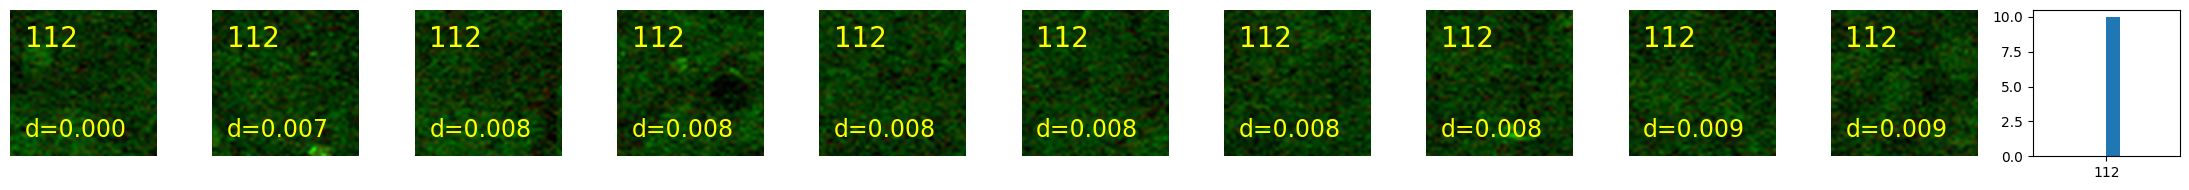
\includegraphics[width=\linewidth]{pediatric-brain-tumours/images/simclr-nn-5.png} \\
        \midrule
        \raisebox{1.6\normalbaselineskip}[0pt][0pt]{\rotatebox[origin=c]{90}{\tiny ImageNet}} & 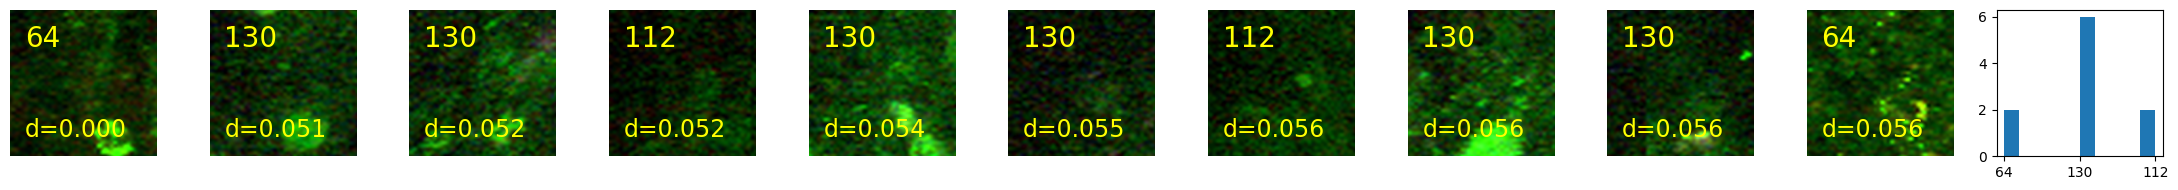
\includegraphics[width=\linewidth]{pediatric-brain-tumours/images/imagenet-nn-6.png} \\
        \raisebox{1.6\normalbaselineskip}[0pt][0pt]{\rotatebox[origin=c]{90}{\tiny SimCLR}} & 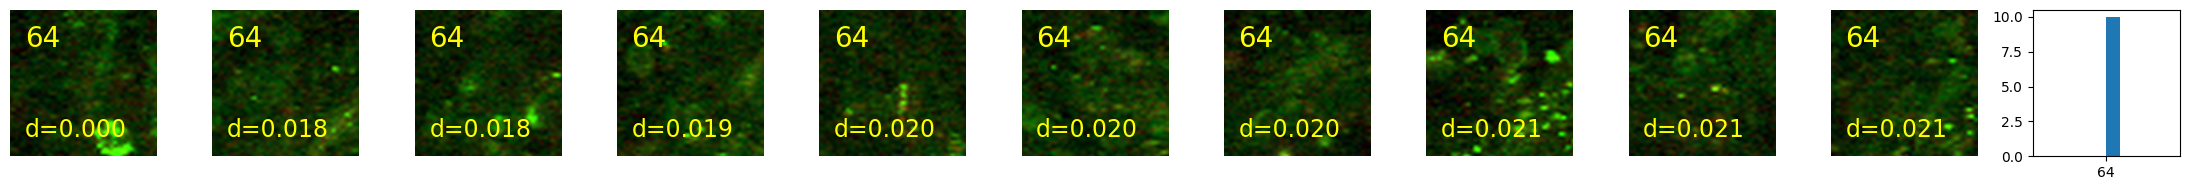
\includegraphics[width=\linewidth]{pediatric-brain-tumours/images/simclr-nn-6.png} \\
        \midrule
        \raisebox{1.6\normalbaselineskip}[0pt][0pt]{\rotatebox[origin=c]{90}{\tiny ImageNet}} & 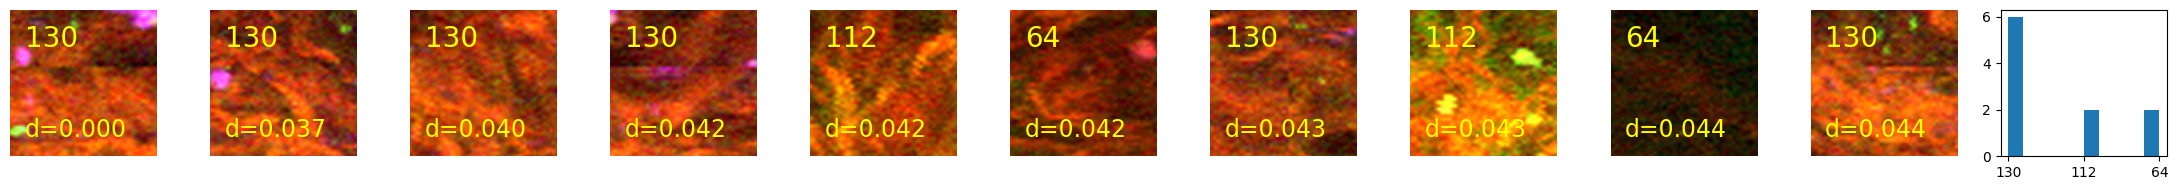
\includegraphics[width=\linewidth]{pediatric-brain-tumours/images/imagenet-nn-7.png} \\
        \raisebox{1.6\normalbaselineskip}[0pt][0pt]{\rotatebox[origin=c]{90}{\tiny SimCLR}} & 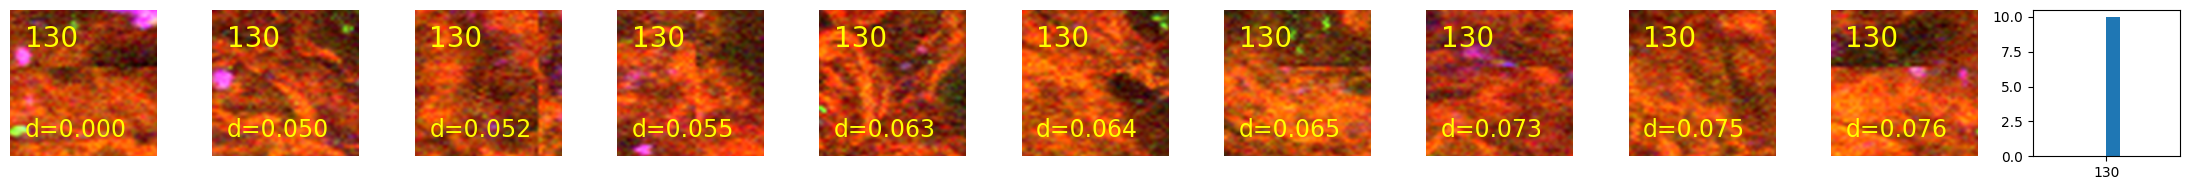
\includegraphics[width=\linewidth]{pediatric-brain-tumours/images/simclr-nn-7.png}
    \end{tabular}
    \caption[Nearest neighbors visualization in image space]{
        Nearest neighbors visualization in image space.
        Neighbors were first calculated in feature space and their corresponding tiles are plotted.
        Every first row after dividers are calculated using the ImageNet pretrained backbone.
        Every second row is calculated using the SimCLR pretrained backbone.
        Bottom left shows the Euclidean distance ($d$) with respect to the target image in the first column.
        The last column shows the distribution of cases for the first 10 nearest neighbors.
    }
    \label{fig:nearest-neighbours-image-space}
\end{figure*}

\paragraph{T-SNE feature embedding}
To further see how the features are distributed, the higher dimensional feature vectors of the validation set of fold 0 are projected onto two-dimensions using t-SNE at multiple perplexities.
The t-SNE embeddings are shown three times with different colors for diagnosis, case and image in \cref{fig:tsne-features}.

\begin{figure*}
    \centering
    \begin{tabular}[\linewidth]{c}
    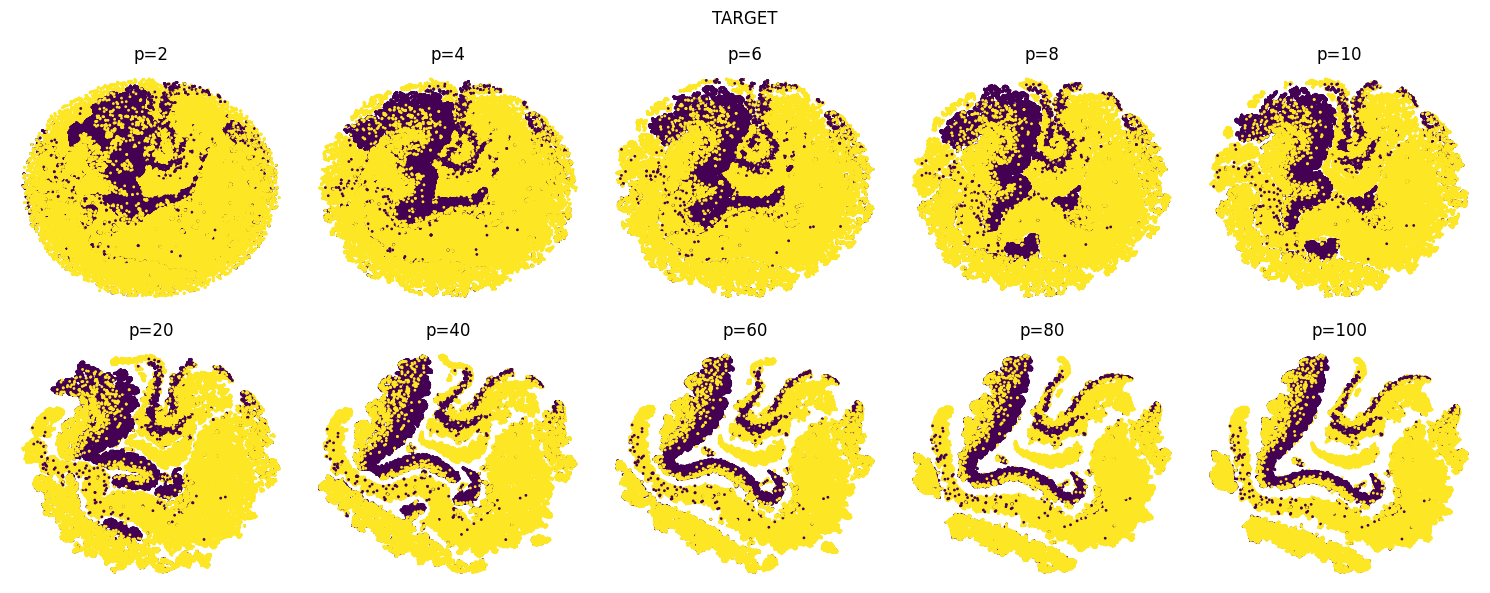
\includegraphics[width=\linewidth]{pediatric-brain-tumours/images/target-tsne.png} \\
    \midrule
    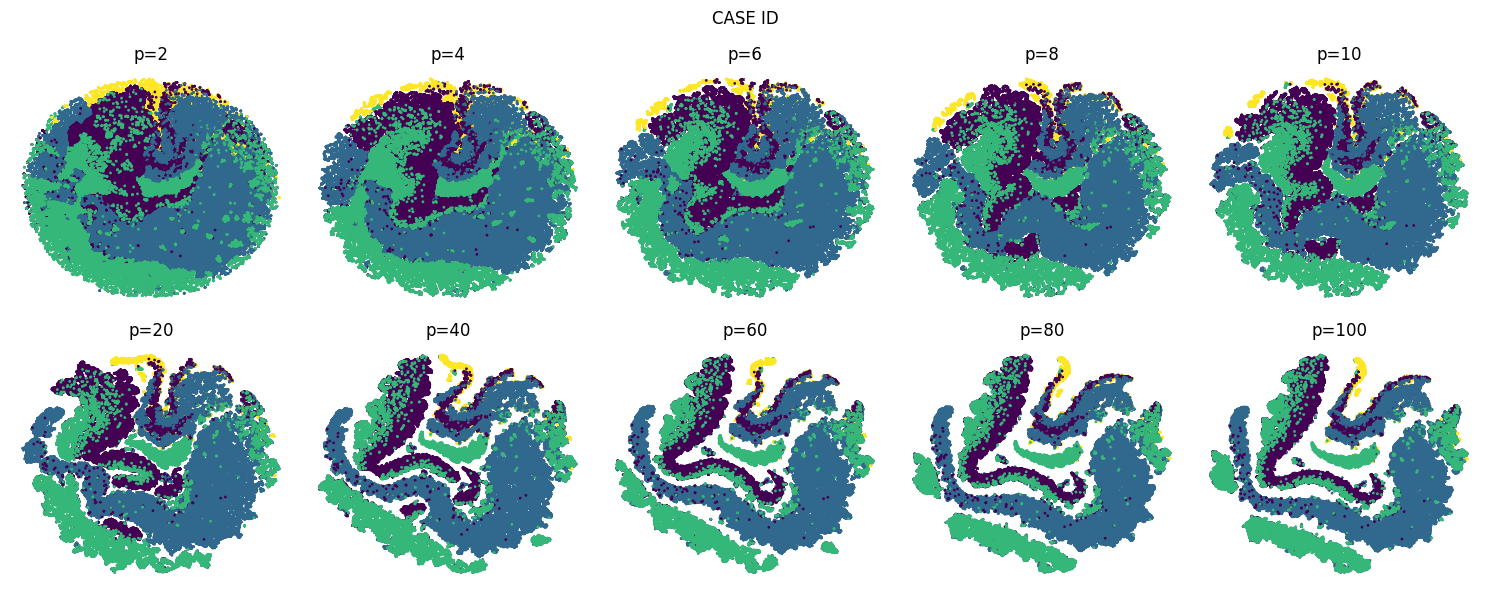
\includegraphics[width=\linewidth]{pediatric-brain-tumours/images/case-tsne.png} \\
    \midrule
    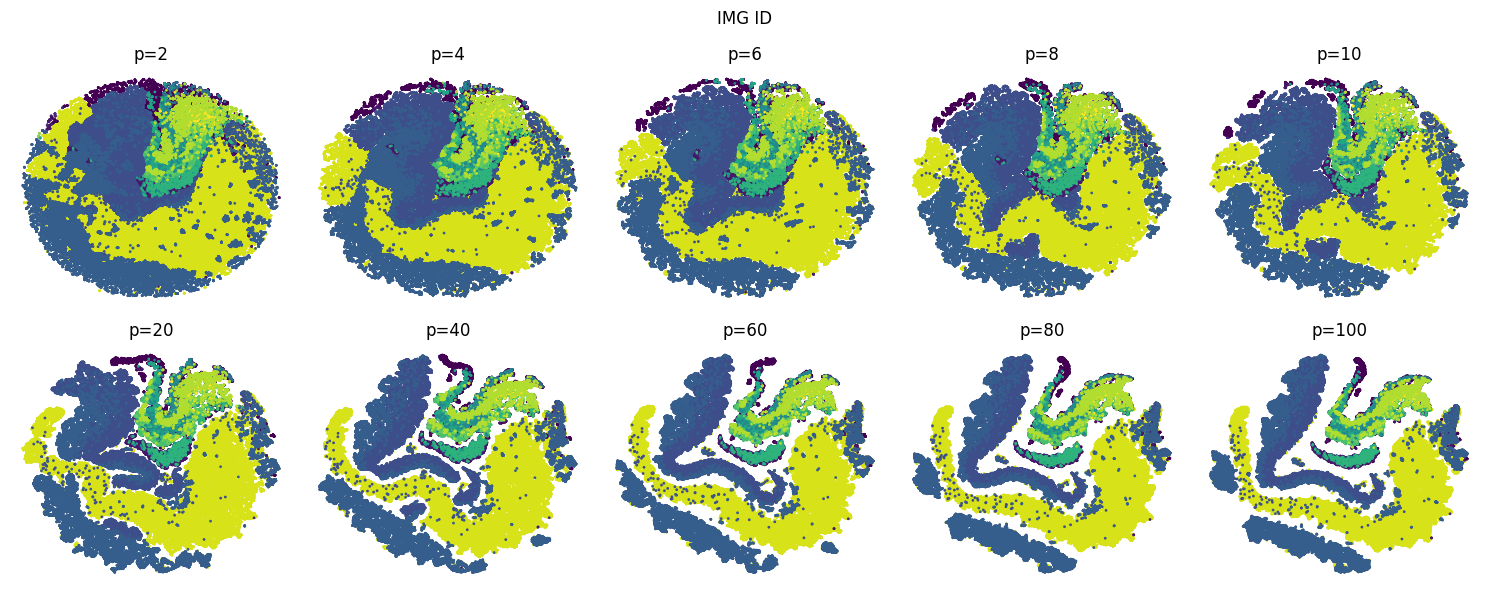
\includegraphics[width=\linewidth]{pediatric-brain-tumours/images/img-tsne.png}
    \end{tabular}
    \caption[T-SNE projections of features]{
        Features of the validation set of fold 0 visualized in two-dimensional t-SNE projections at perplexities $p=\{2,\,4,\,6,\,8,\,10,\,20,\,40,\,60,\,80,\,100\}$.
        Points are colored by diagnosis, case and image.
    }
    \label{fig:tsne-features}
\end{figure*}

\subsubsection{MIL}

The cross entropy loss for all folds for the SimCLR + CCMIL classifier training is shown in \cref{fig:simclr-ccmil-loss}.
Loss curves for the VarMIL models are similar.
Note the validation loss of fold 1 diverging from the corresponding training loss, indicating overfitting.

\begin{figure*}
    \centering
    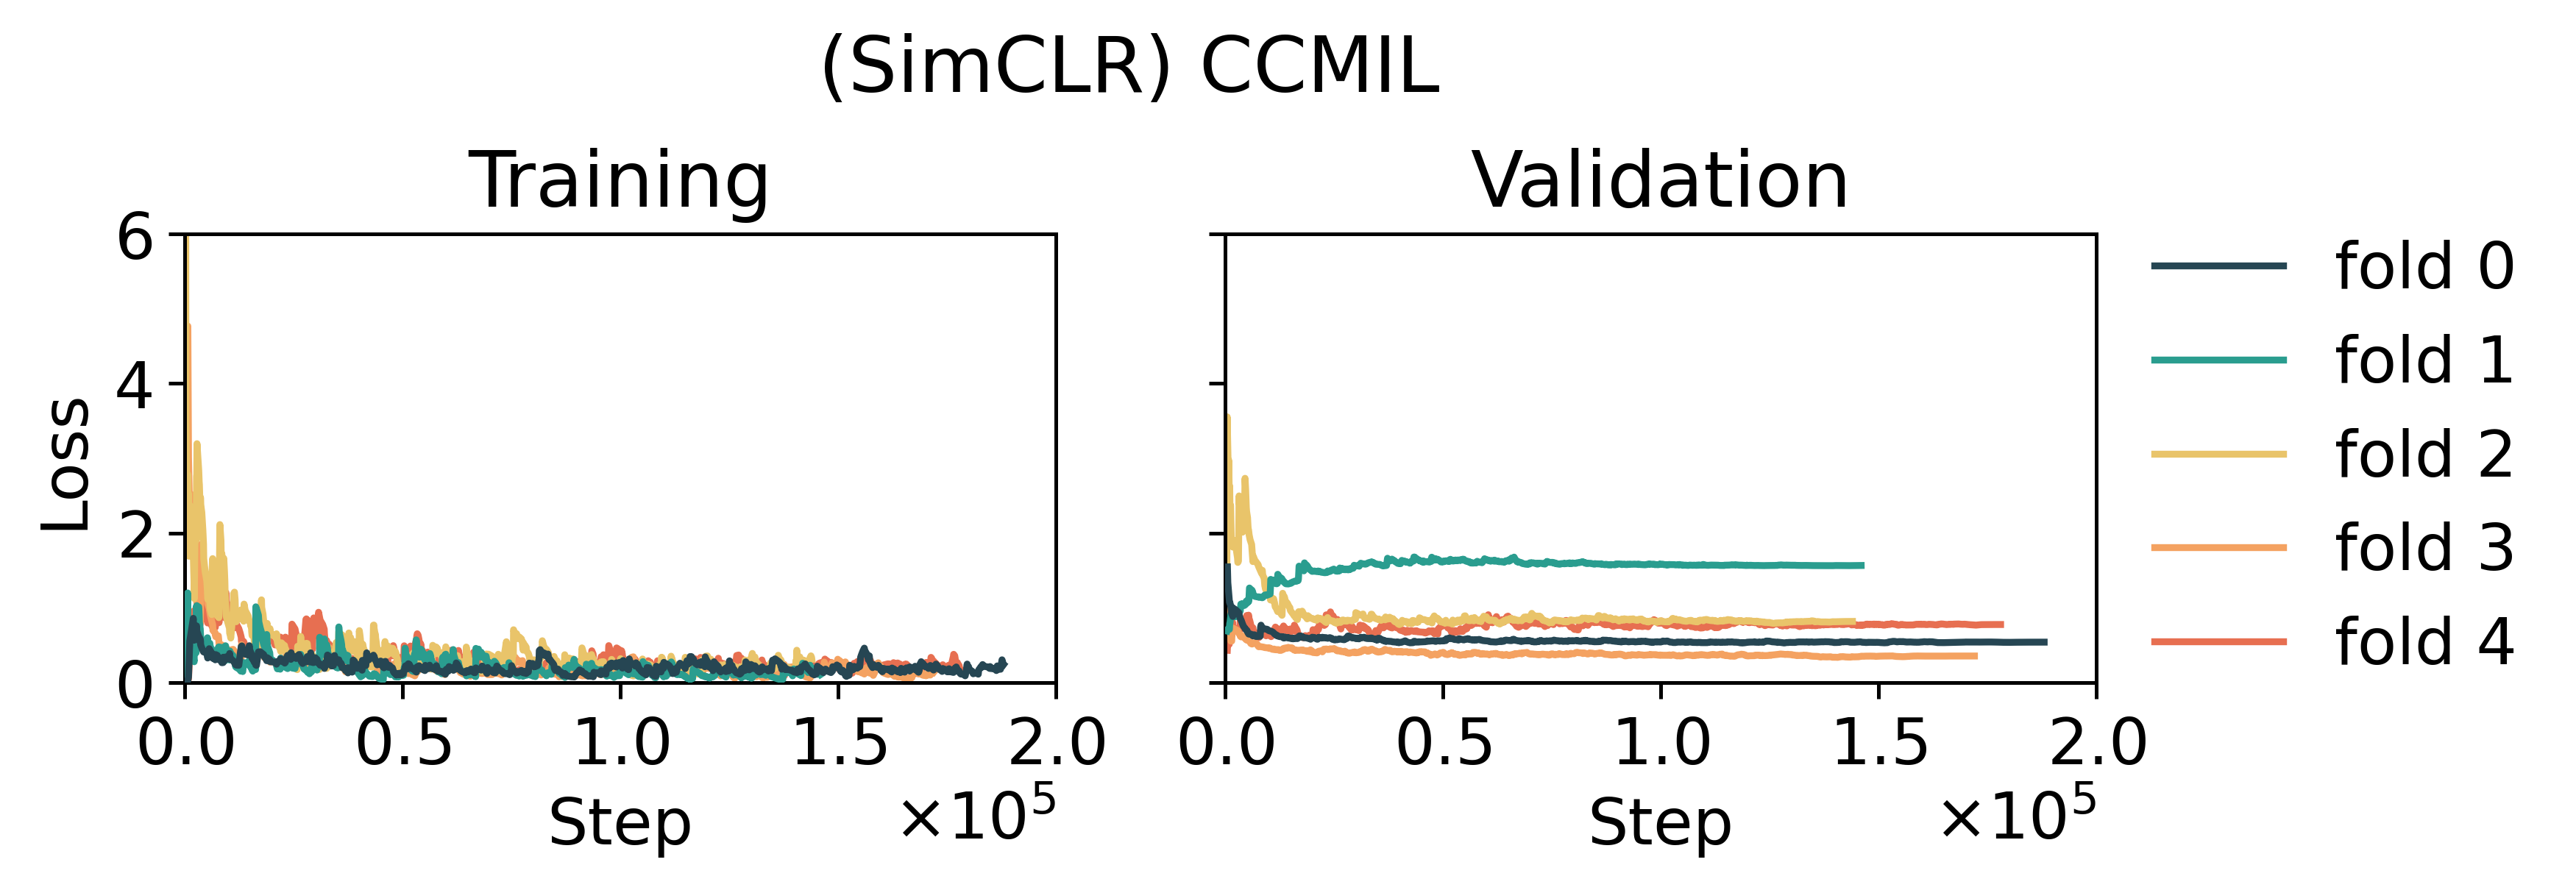
\includegraphics[width=\linewidth]{pediatric-brain-tumours/images/simclr+ccmil-loss.png}
    \caption[Training loss CCMIL]{
        Cross entropy loss for training the classifier of the SimCLR + CCMIL model.
        The loss for the training and validation all five folds are shown.
    }
    \label{fig:simclr-ccmil-loss}
\end{figure*}

The ROC, PR, and PRG curves of the model applied on the test set are shown in \cref{fig:roc-pr-prg}.
The mean AUC, AUPR, and AUPRG are summarized in \cref{tab:performance}.

When making conclusions on performance based on PR curves, one might find that fold 1 and 2 of the SimCLR + VarMIL model perform comparably.
Eliminating data outcome bias with the PRG curve shows a significant difference between those models where fold 1 is performing worse than the always positive classifiers.
Based on the ROC curve, one might conclude that the model of fold 2 only performs marginally better than that of fold 1.
% The PRG curve makes it immediately clear what models perform better than the baseline classifier.
% When just using the ROC curve without the always positive classifier baselines, one would quickly conclude that 

\begin{figure*}
    \centering
    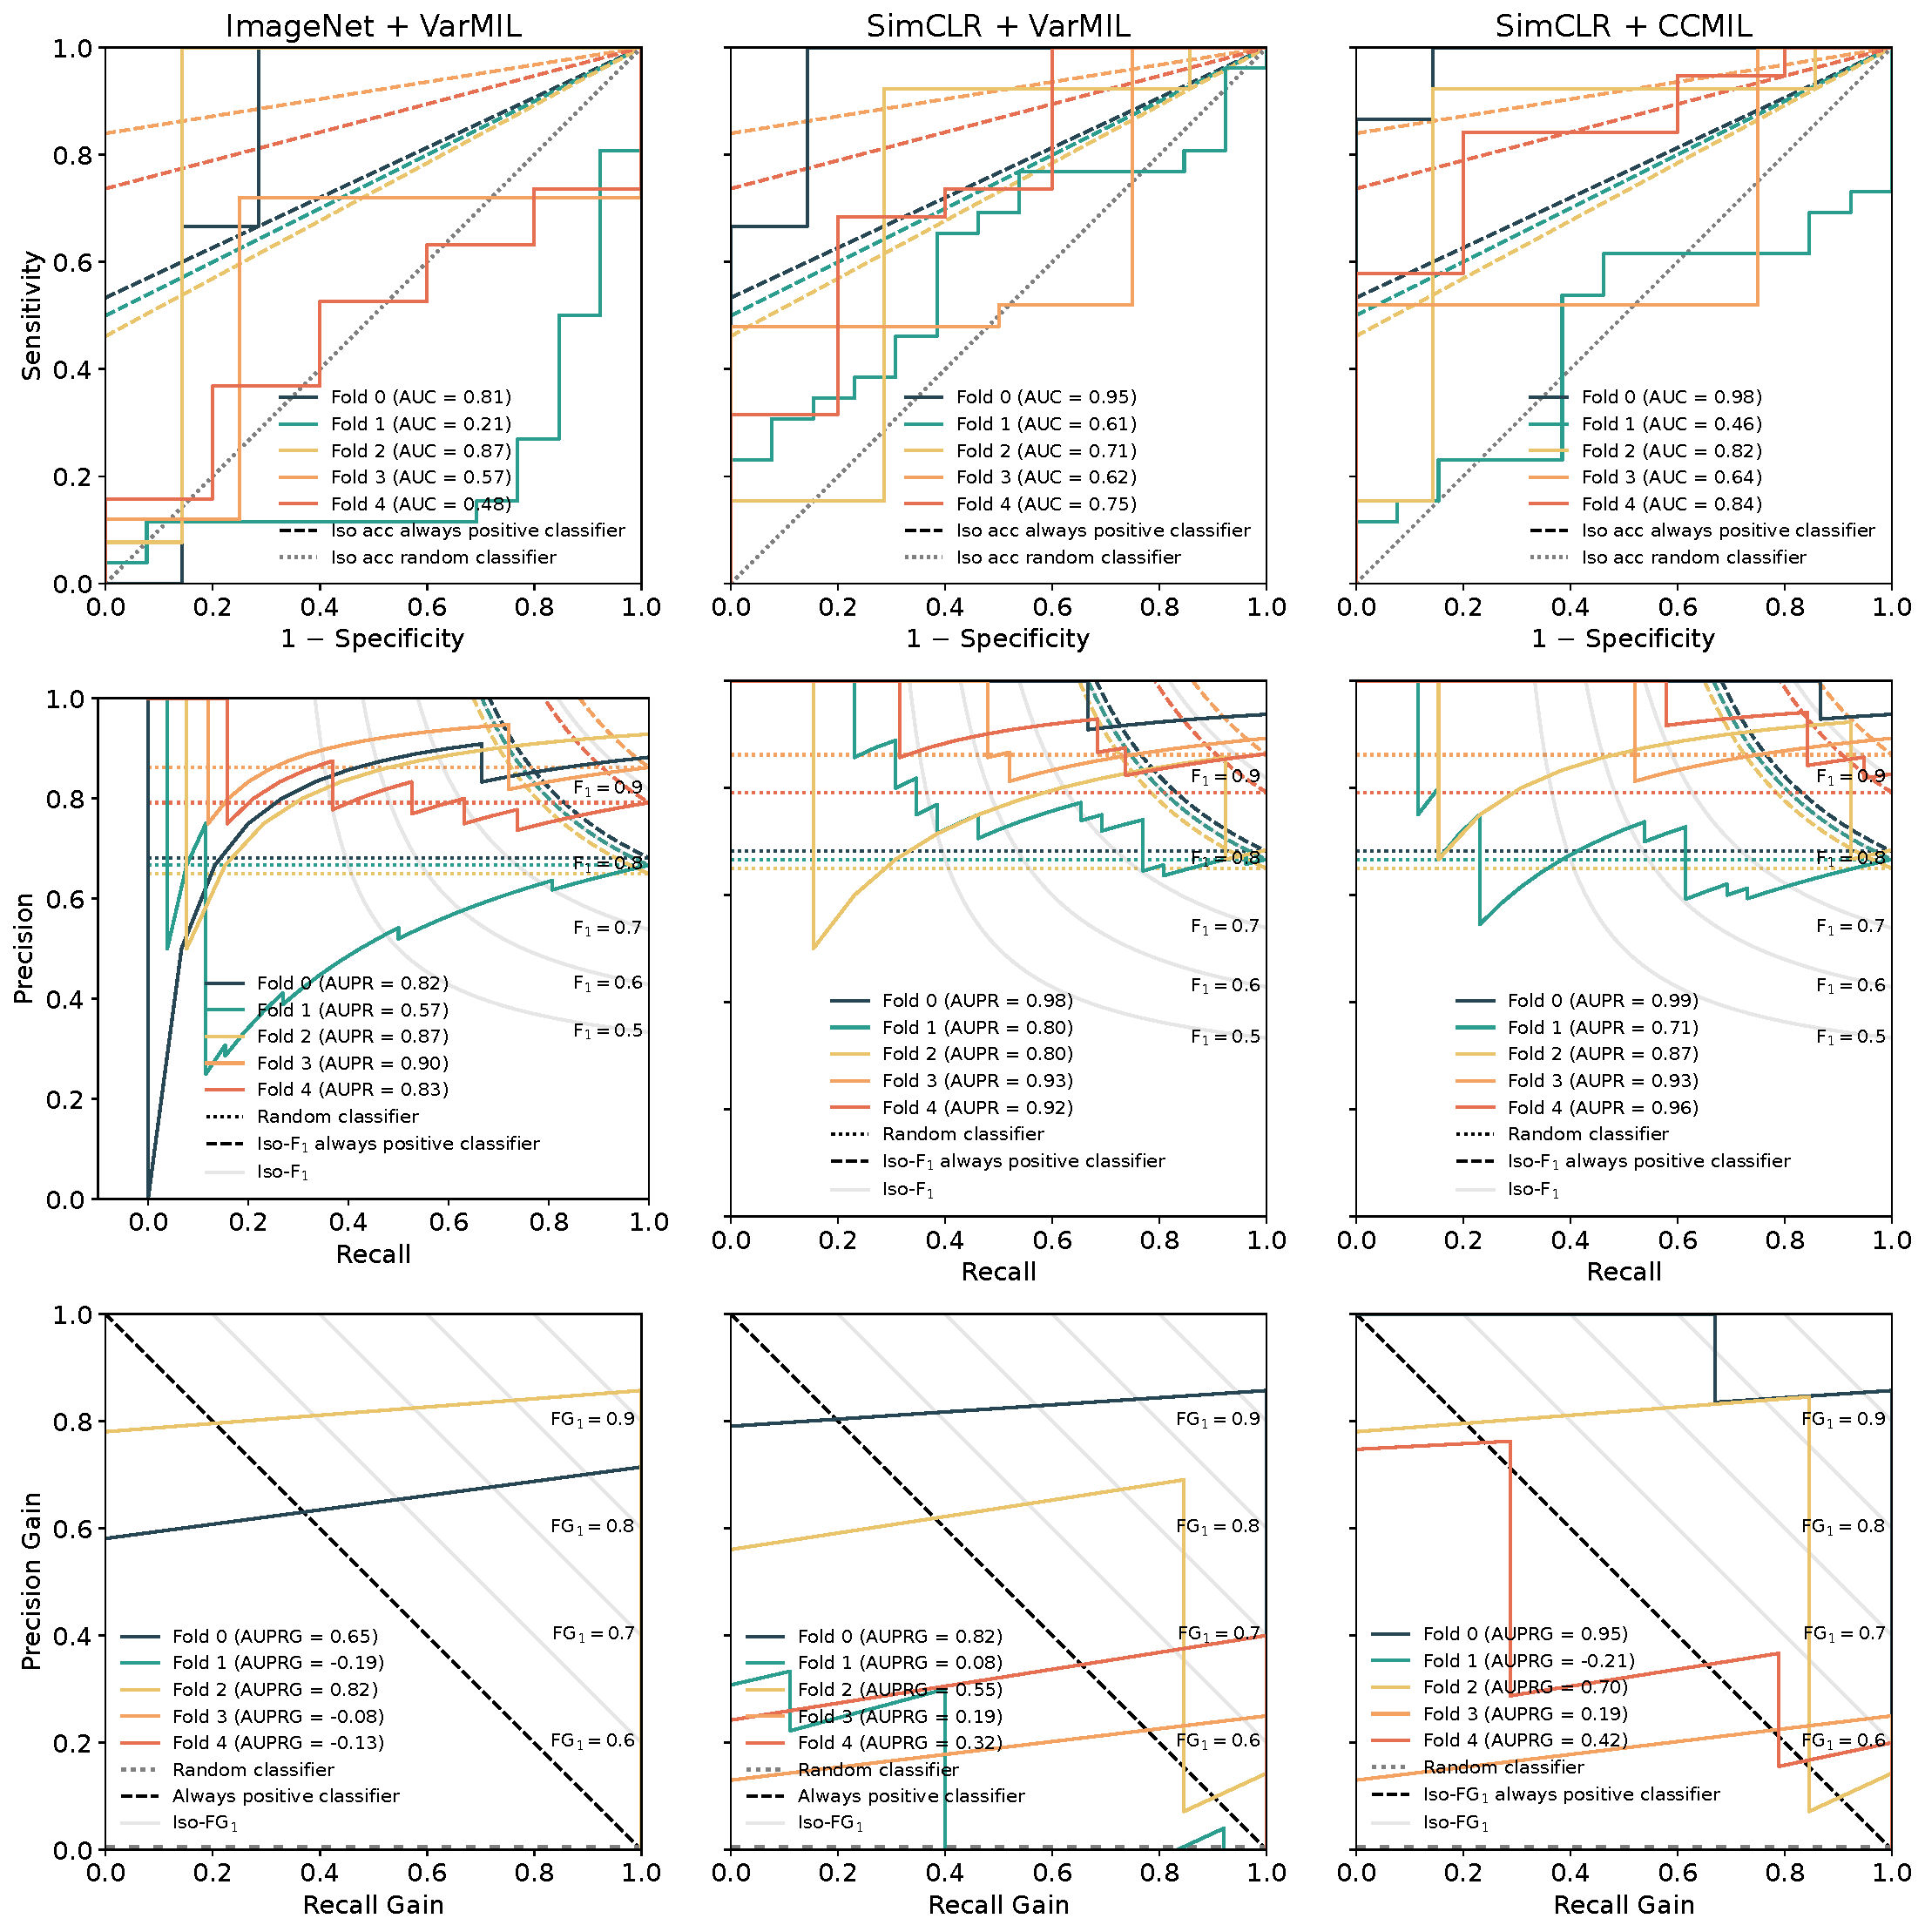
\includegraphics[width=\linewidth]{pediatric-brain-tumours/images/all.pdf}
    \caption[ROC, PR, and PRG]{
        ROC, PR, and PRG curves of the model applied on the test set.
        Top row: ROC curves (color solid) for \emph{feature extractor} + \emph{classifier} with iso-accuracy lines of the always positive classifier (color dashed) and a random classifier (dotted) are shown.
        The iso-accuracies all go through a classifier with $\mathrm{sensitivity} = 1 - \textrm{specificity} = 1$, but are non-universal.
        The iso-accuracy of a random classifier is universal.
        For every fold, the AUC is reported.
        Middle row: PR curves (color solid) with iso-$F_1$ lines of the always positive classifier (color dashed) and a random classifier (color dotted).
        The iso-$F_1$ curves go to the upper right corner for increasing $F_1$.
        The iso-$F_1$ lines of the random classifiers go to 1 for increasing bias to pilocytic astrocytoma examples.
        Iso-$F_1$ lines are not universal.
        For every fold, the AUPR is reported.
        Bottom row: PRG curves (color solid) with iso-$FG_1$ lines (solid gray).
        The precision gain of the random classifier (dotted on $\mathrm{precision\,gain} = 0$) and the always positive classifier baseline (dashed) are universal.
        Points on the PRG curves with $\mathrm{precision\,gain} < 0$ or $\mathrm{recall\,gain} < 0$ are not shown.
        For every fold, the AUPRG is reported.
    }
    \label{fig:roc-pr-prg}
\end{figure*}

\begin{table*}
    \caption[AUC, AUPR, and AUPRG]{AUC, AUPR, and AUPRG with \qty{95}{\percent} CI of three different models applied to the validation and test set.
    No value is significantly different.}
    \label{tab:performance}
    \begin{tabular*}{\linewidth}{@{\extracolsep{\fill}}*{7}{c}}
        \toprule
        \multirow{2}{*}{Model} & \multicolumn{3}{c}{Validation} & \multicolumn{3}{c}{Test} \\
        \cmidrule{2-4} \cmidrule{5-7}
        & AUC & AUPR & AUPRG & AUC & AUPR & AUPRG \\
        \midrule
        ImageNet + VarMIL & \num{0.86 \pm 0.15} & \num{0.96 \pm 0.04} & \num{0.57 \pm 0.43} & \num{0.59 \pm 0.33} & \num{0.80 \pm 0.16} & \num{0.21 \pm 0.60} \\
        SimCLR + VarMIL & \num{0.69 \pm 0.24} & \num{0.89 \pm 0.08} & \num{0.28 \pm 0.37} & \num{0.73 \pm 0.17} & \num{0.88 \pm 0.10} & \num{0.39 \pm 0.37} \\
        SimCLR + CCMIL & \num{0.71 \pm 0.28} & \num{0.90 \pm 0.10} & \num{0.34 \pm 0.54} & \num{0.75 \pm 0.25} & \num{0.89 \pm 0.14} & \num{0.41 \pm 0.56} \\
        \bottomrule
    \end{tabular*}
\end{table*}

The performance of fold 1 is consistently much lower than the other folds, while fold 0 and 2 are consistently higher.
One explanation could be that by coincidence the data quality is lower in fold 1 and higher in fold 0 and 2.
To investigate this, the entropy in the upper part of the power spectrum, and the kurtosis are measured and shown in \cref{fig:data-quality-per-fold}.
Fold 1 shows a wide spread in kurtosis and entropy
The Pearson correlation coefficient ($\mathrm{corr}$) between the test AUPRG and entropy ($h$) and kurtosis ($k$) mean are calculated, like
\begin{align}
    \mathrm{correlation}_h &= \mathbb{E}\left\{[\mathrm{AUPRG} - \mathbb{E}\left(\mathrm{AUPRG} \right)][H - \mathbb{E}\left(H\right)]\right\}, \\
    \mathrm{correlation}_k &= \mathbb{E}\left\{[\mathrm{AUPRG} - \mathbb{E}\left(\mathrm{AUPRG} \right)][K - \mathbb{E}\left(K\right)]\right\}.
\end{align}
Entropy and kurtosis have a small correlation with test AUPRG of 0.19 and -0.15, respectively.

\begin{figure*}
    \centering
    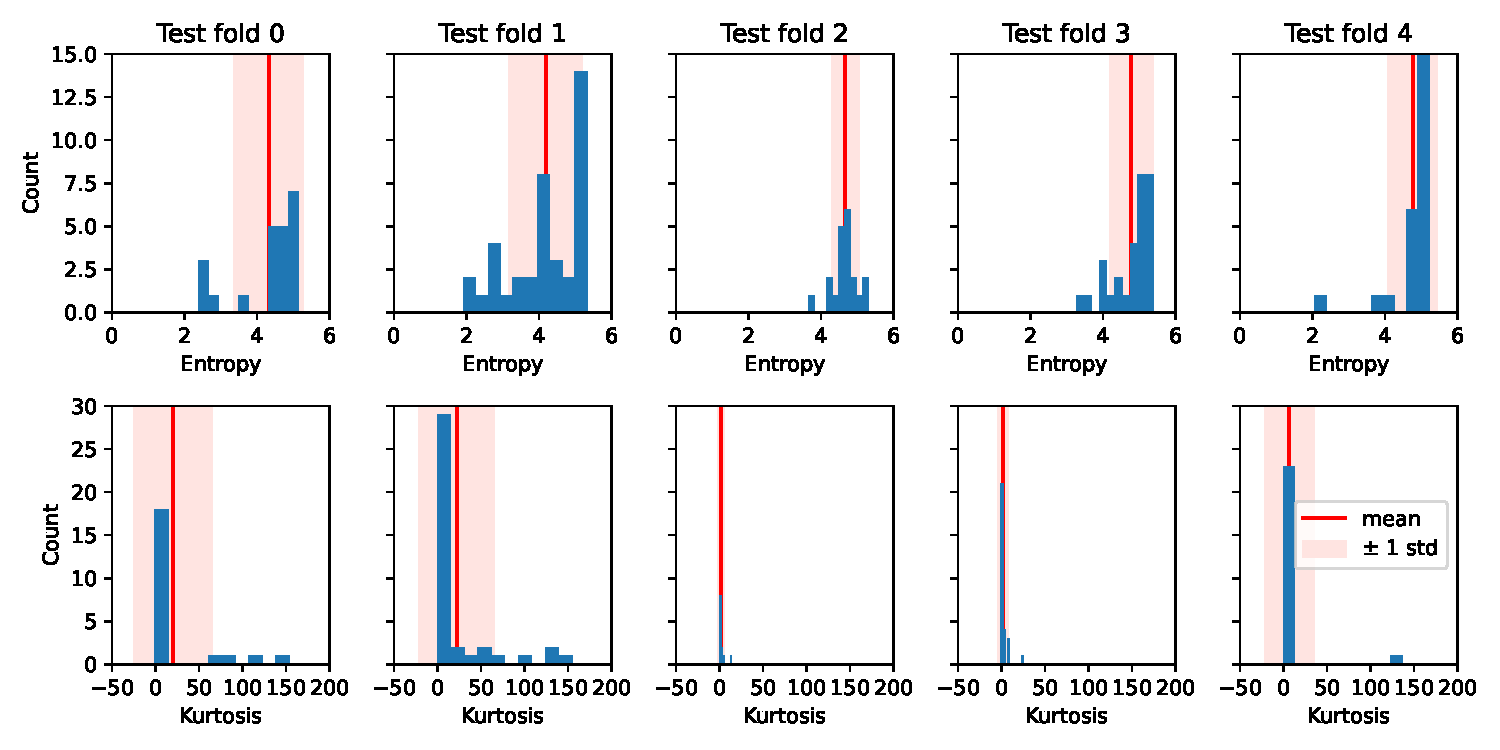
\includegraphics[width=\linewidth]{pediatric-brain-tumours/images/entropy-kurtosis-per-fold-split-test.pdf}
    \caption[Quality of data per test split]{
        Quality of data per test split.
        Top row: entropy of the tail of the power spectrum.
        Bottom row: kurtosis of the tail of the power spectrum.
        The mean (solid) and standard deviation (red region) are shown.
    }
    \label{fig:data-quality-per-fold}
\end{figure*}

\subsection{Explainability}
\subsubsection{Attention weighted images}
Attention weighted images are shown in \cref{fig:a-weighted-images}.
They are created from medulloblastoma and pilocytic astrocytoma data from the test set of fold 0 using the corresponding model.
Only a small portion of the tiles is weighted with a substantial attention weight, resulting in rather dark images.

\begin{figure*}
    \centering
    \begin{tabularx}{\linewidth}{c}
        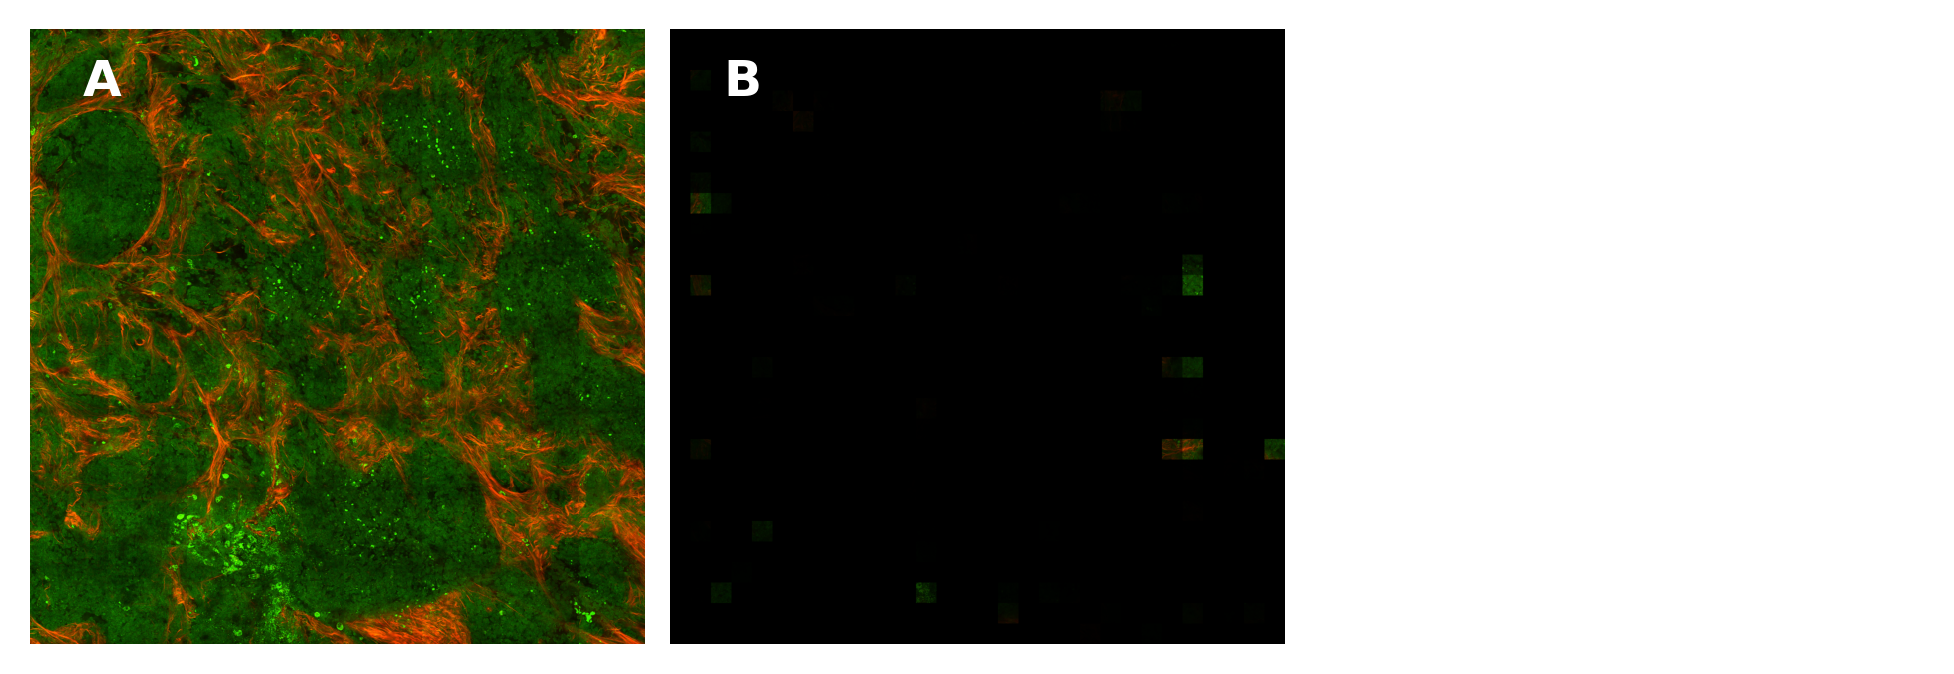
\includegraphics[width=\linewidth]{pediatric-brain-tumours/images/PMC_HHG_36_Hersenen_I-05_8x8_200slow-summary.png} \\
        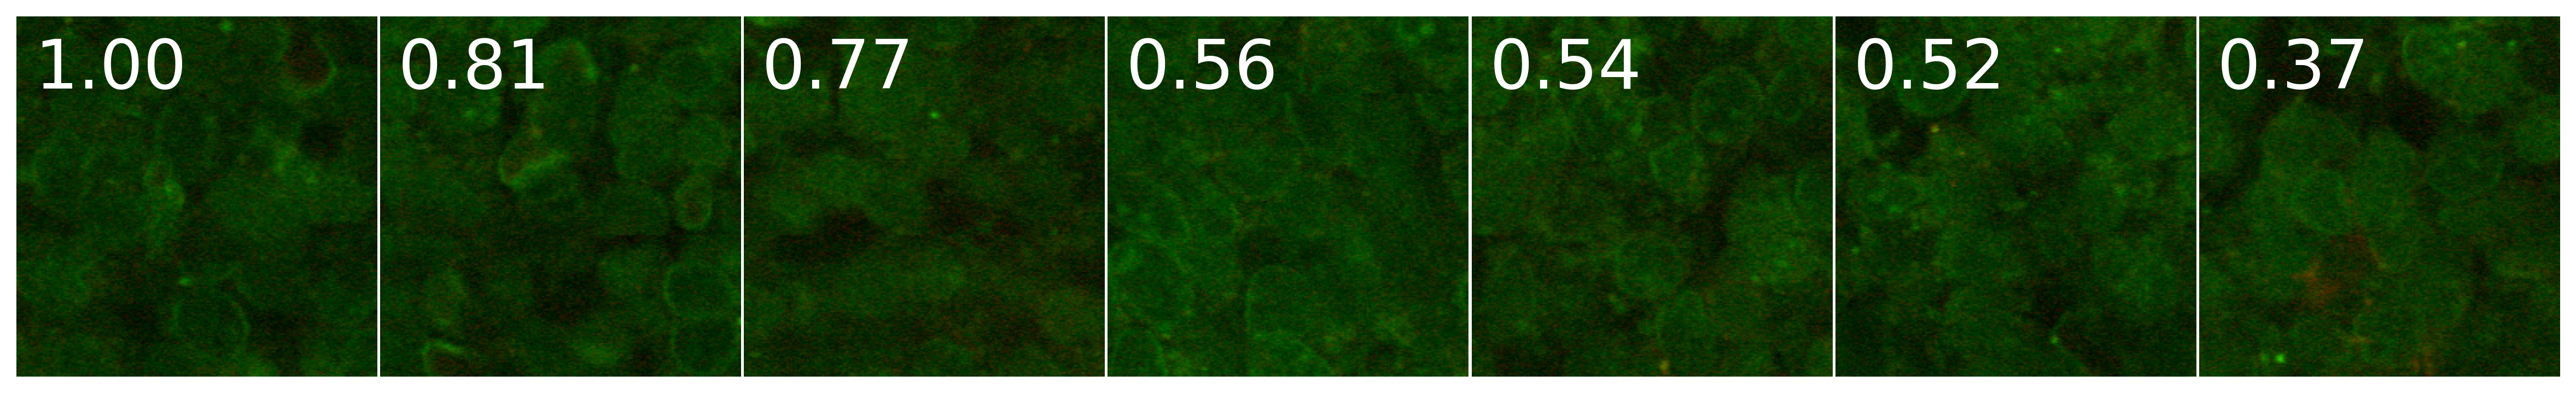
\includegraphics[width=\linewidth]{pediatric-brain-tumours/images/PMC_HHG_36_Hersenen_I-05_8x8_200slow-tiles.png} \\
        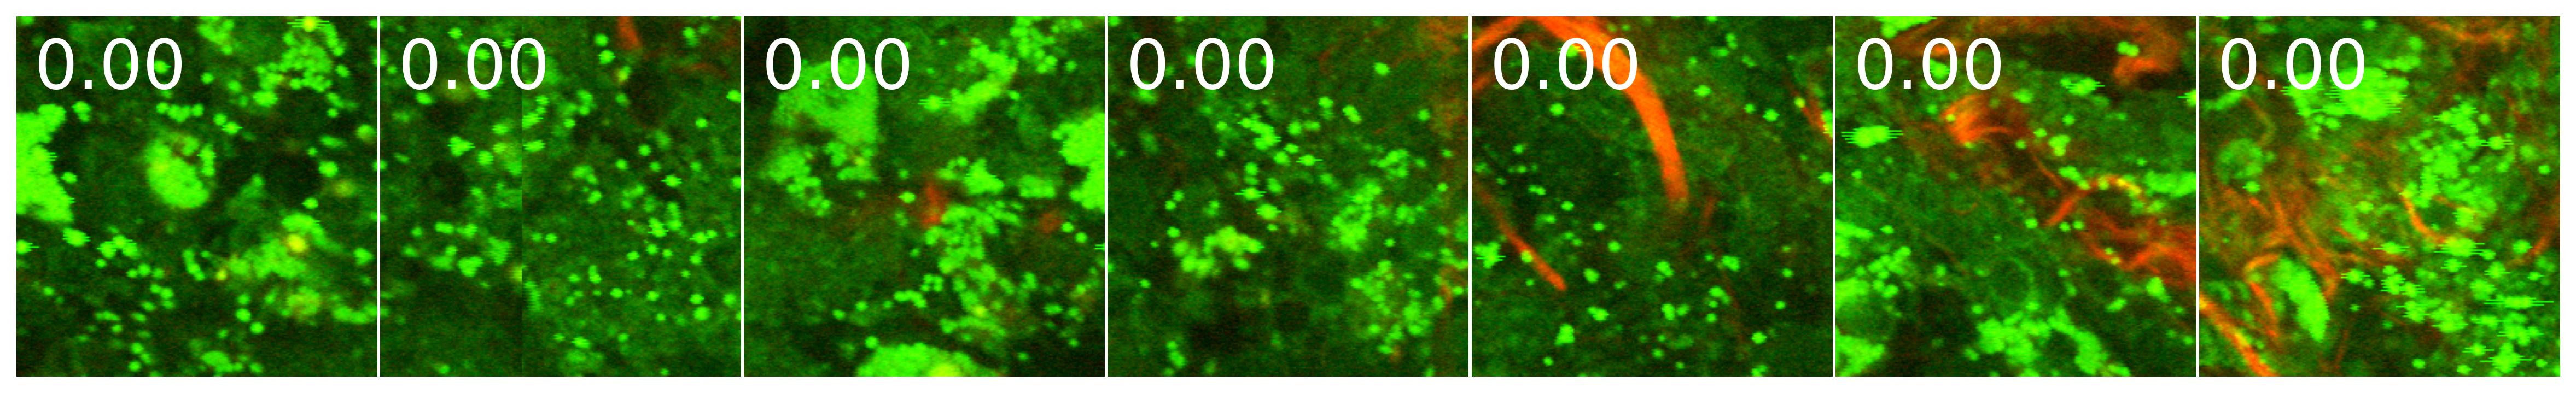
\includegraphics[width=\linewidth]{pediatric-brain-tumours/images/PMC_HHG_36_Hersenen_I-05_8x8_200slow-tiles-low-a.png} \\
        \midrule
        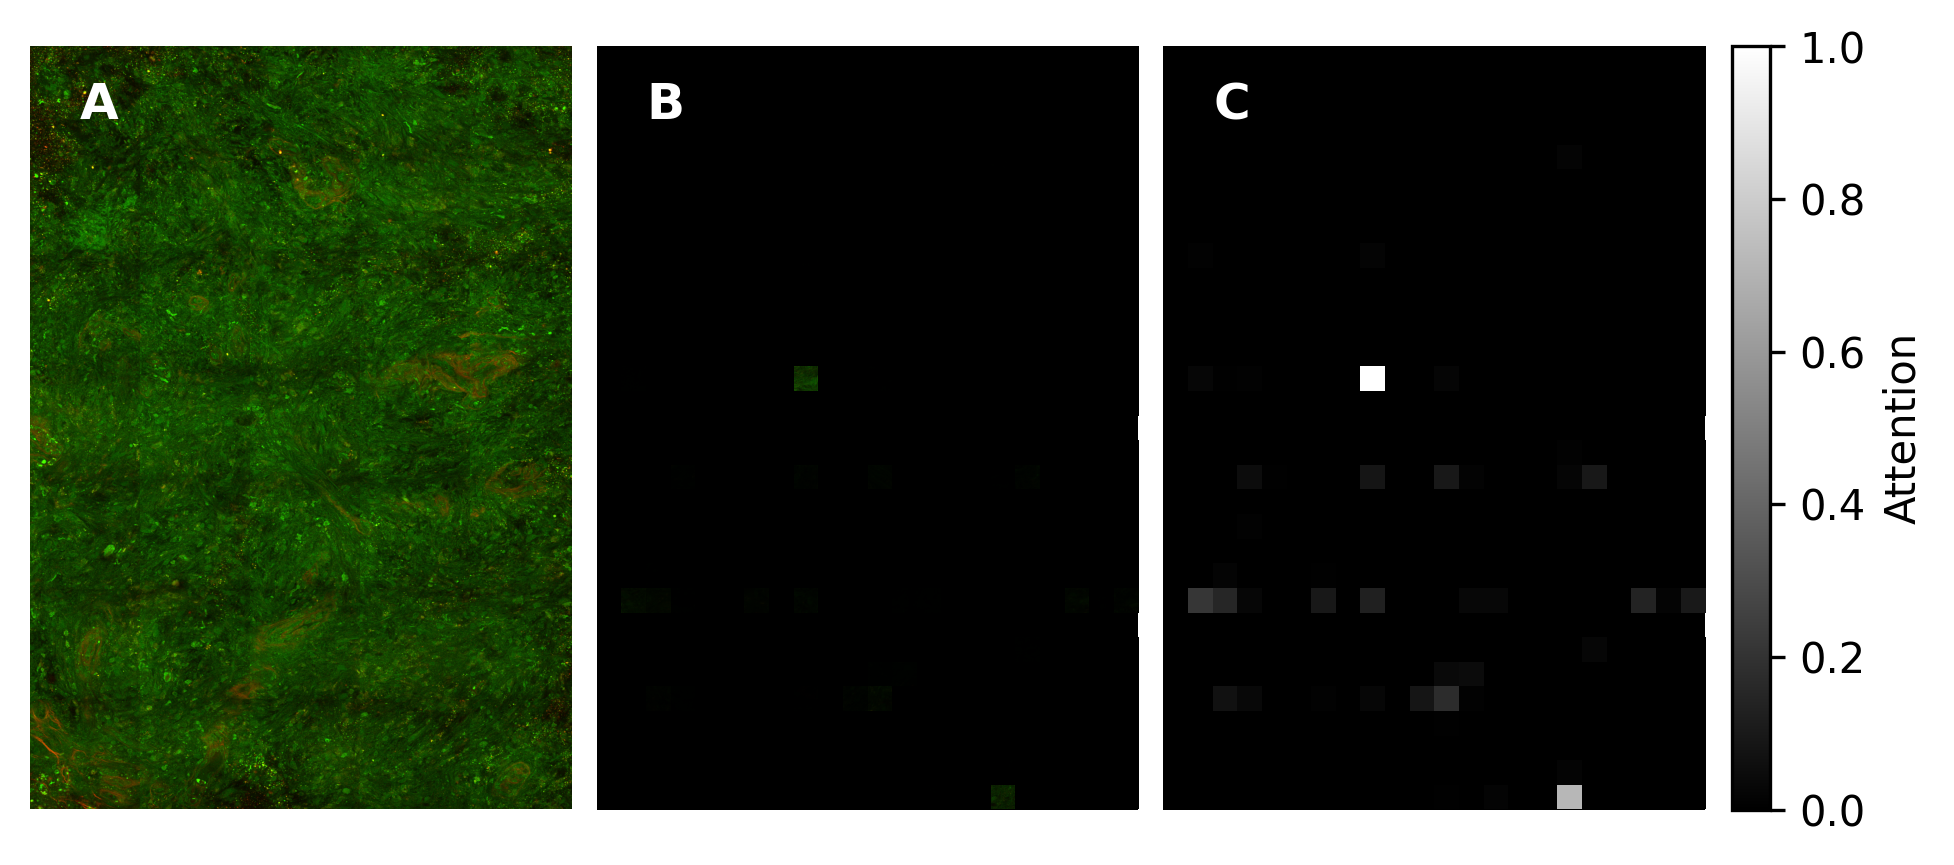
\includegraphics[width=\linewidth]{pediatric-brain-tumours/images/PMC_HHG_32_Hersenen_I-05_5x7_200slow-summary.png} \\
        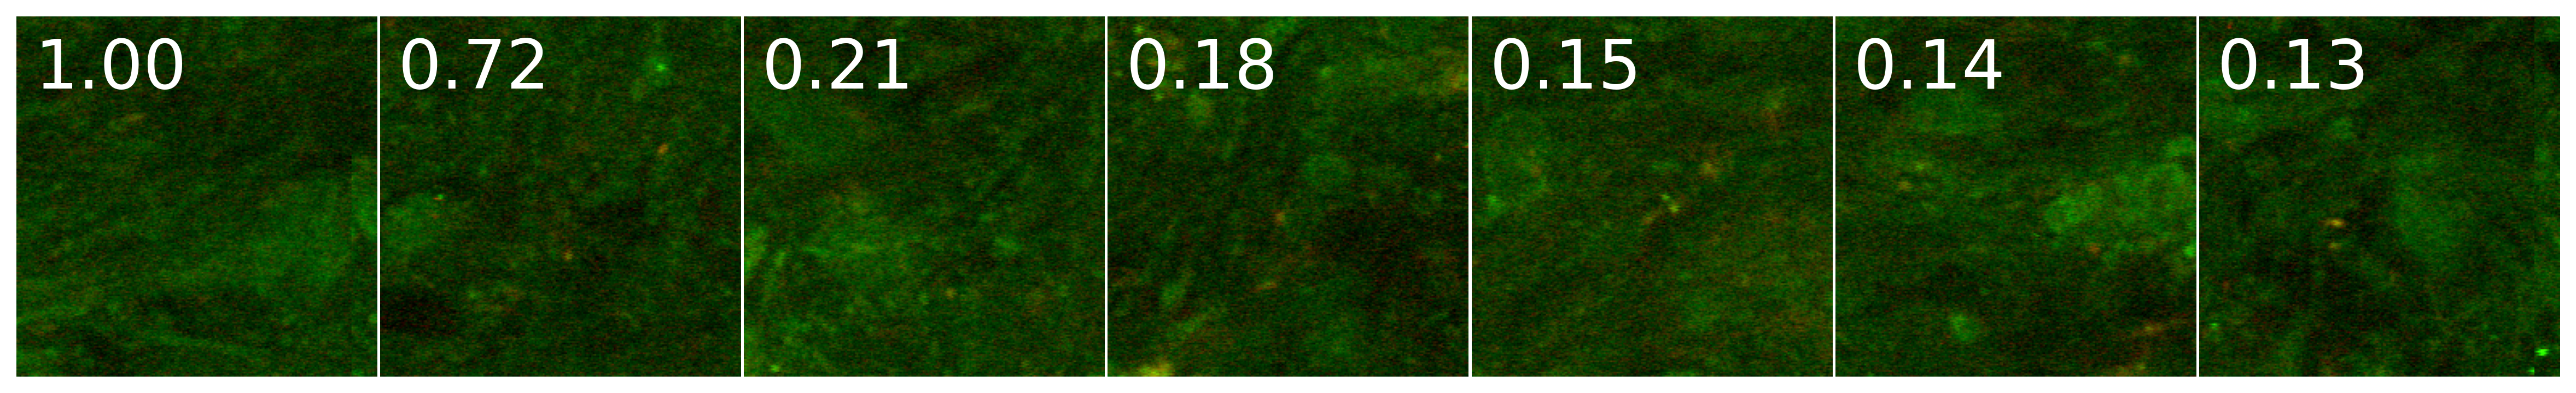
\includegraphics[width=\linewidth]{pediatric-brain-tumours/images/PMC_HHG_32_Hersenen_I-05_5x7_200slow-tiles.png} \\
        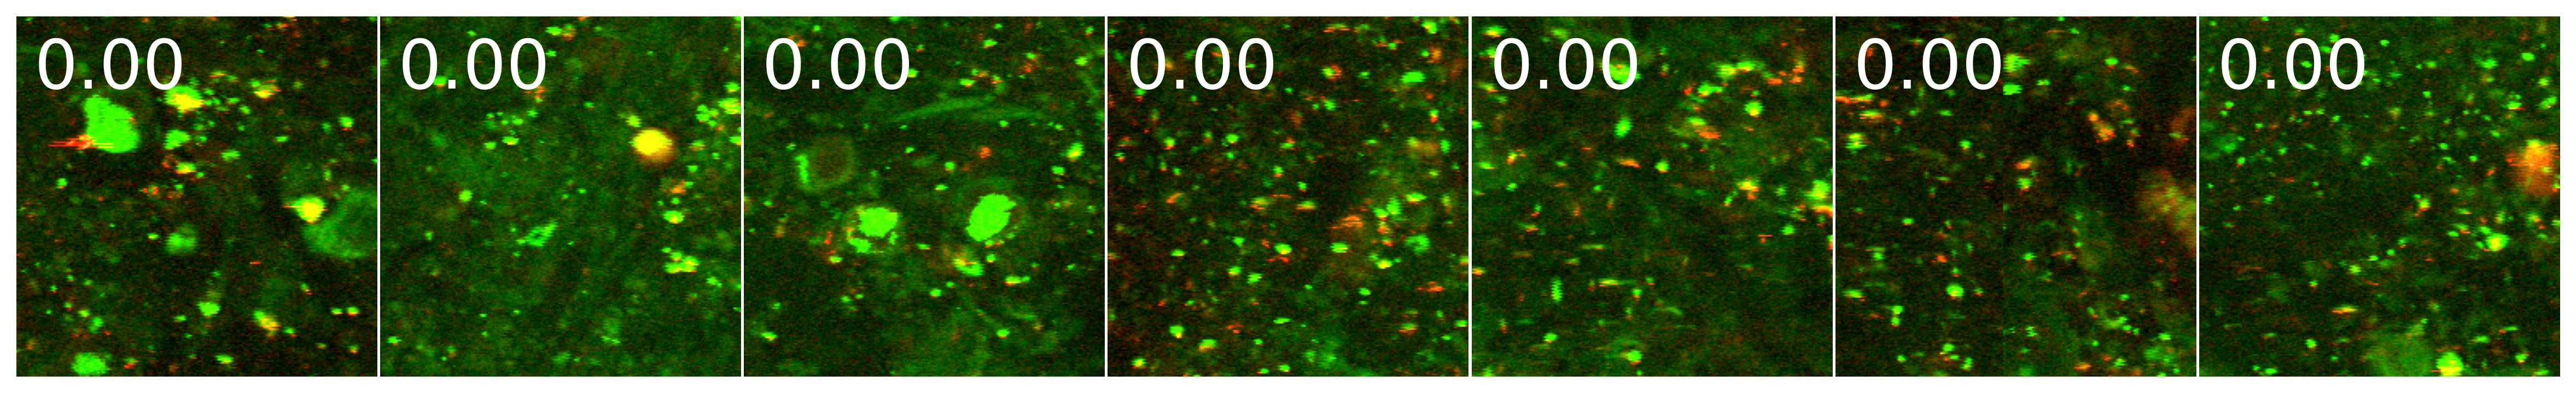
\includegraphics[width=\linewidth]{pediatric-brain-tumours/images/PMC_HHG_32_Hersenen_I-05_5x7_200slow-tiles-low-a.png}
    \end{tabularx}
    \caption[Attention weighted images]{
        Attention weighted images.
        Tiles are multiplied with min-max-normalized attention weights.
        Top: medulloblastoma (prediction score = 0.76).
        Bottom: pilocytic astrocytoma (prediction score = 0.81).
        First rows show the original image (A), the attention weighted image (B) and the local attentions (linear grayscale) compared with pathologist annotations (green) (C).
        Second and third rows show the tiles with the highest and lowest attention weights, respectively.
        The corresponding normalized attention weight is printed.
    }
    \label{fig:a-weighted-images}
\end{figure*}

\subsubsection{Location embeddings}
A t-SNE projection of the location embeddings is shown in \cref{fig:tsne-cc}.
Texts seem grouped (\eg, "ventricle", "posterior cranial fossa", "cereb-", "brainstem", "lobe").
The groupings are visualized by fitting a Gaussian mixture model with six components to the t-SNE projections.

\begin{figure}
    \centering
    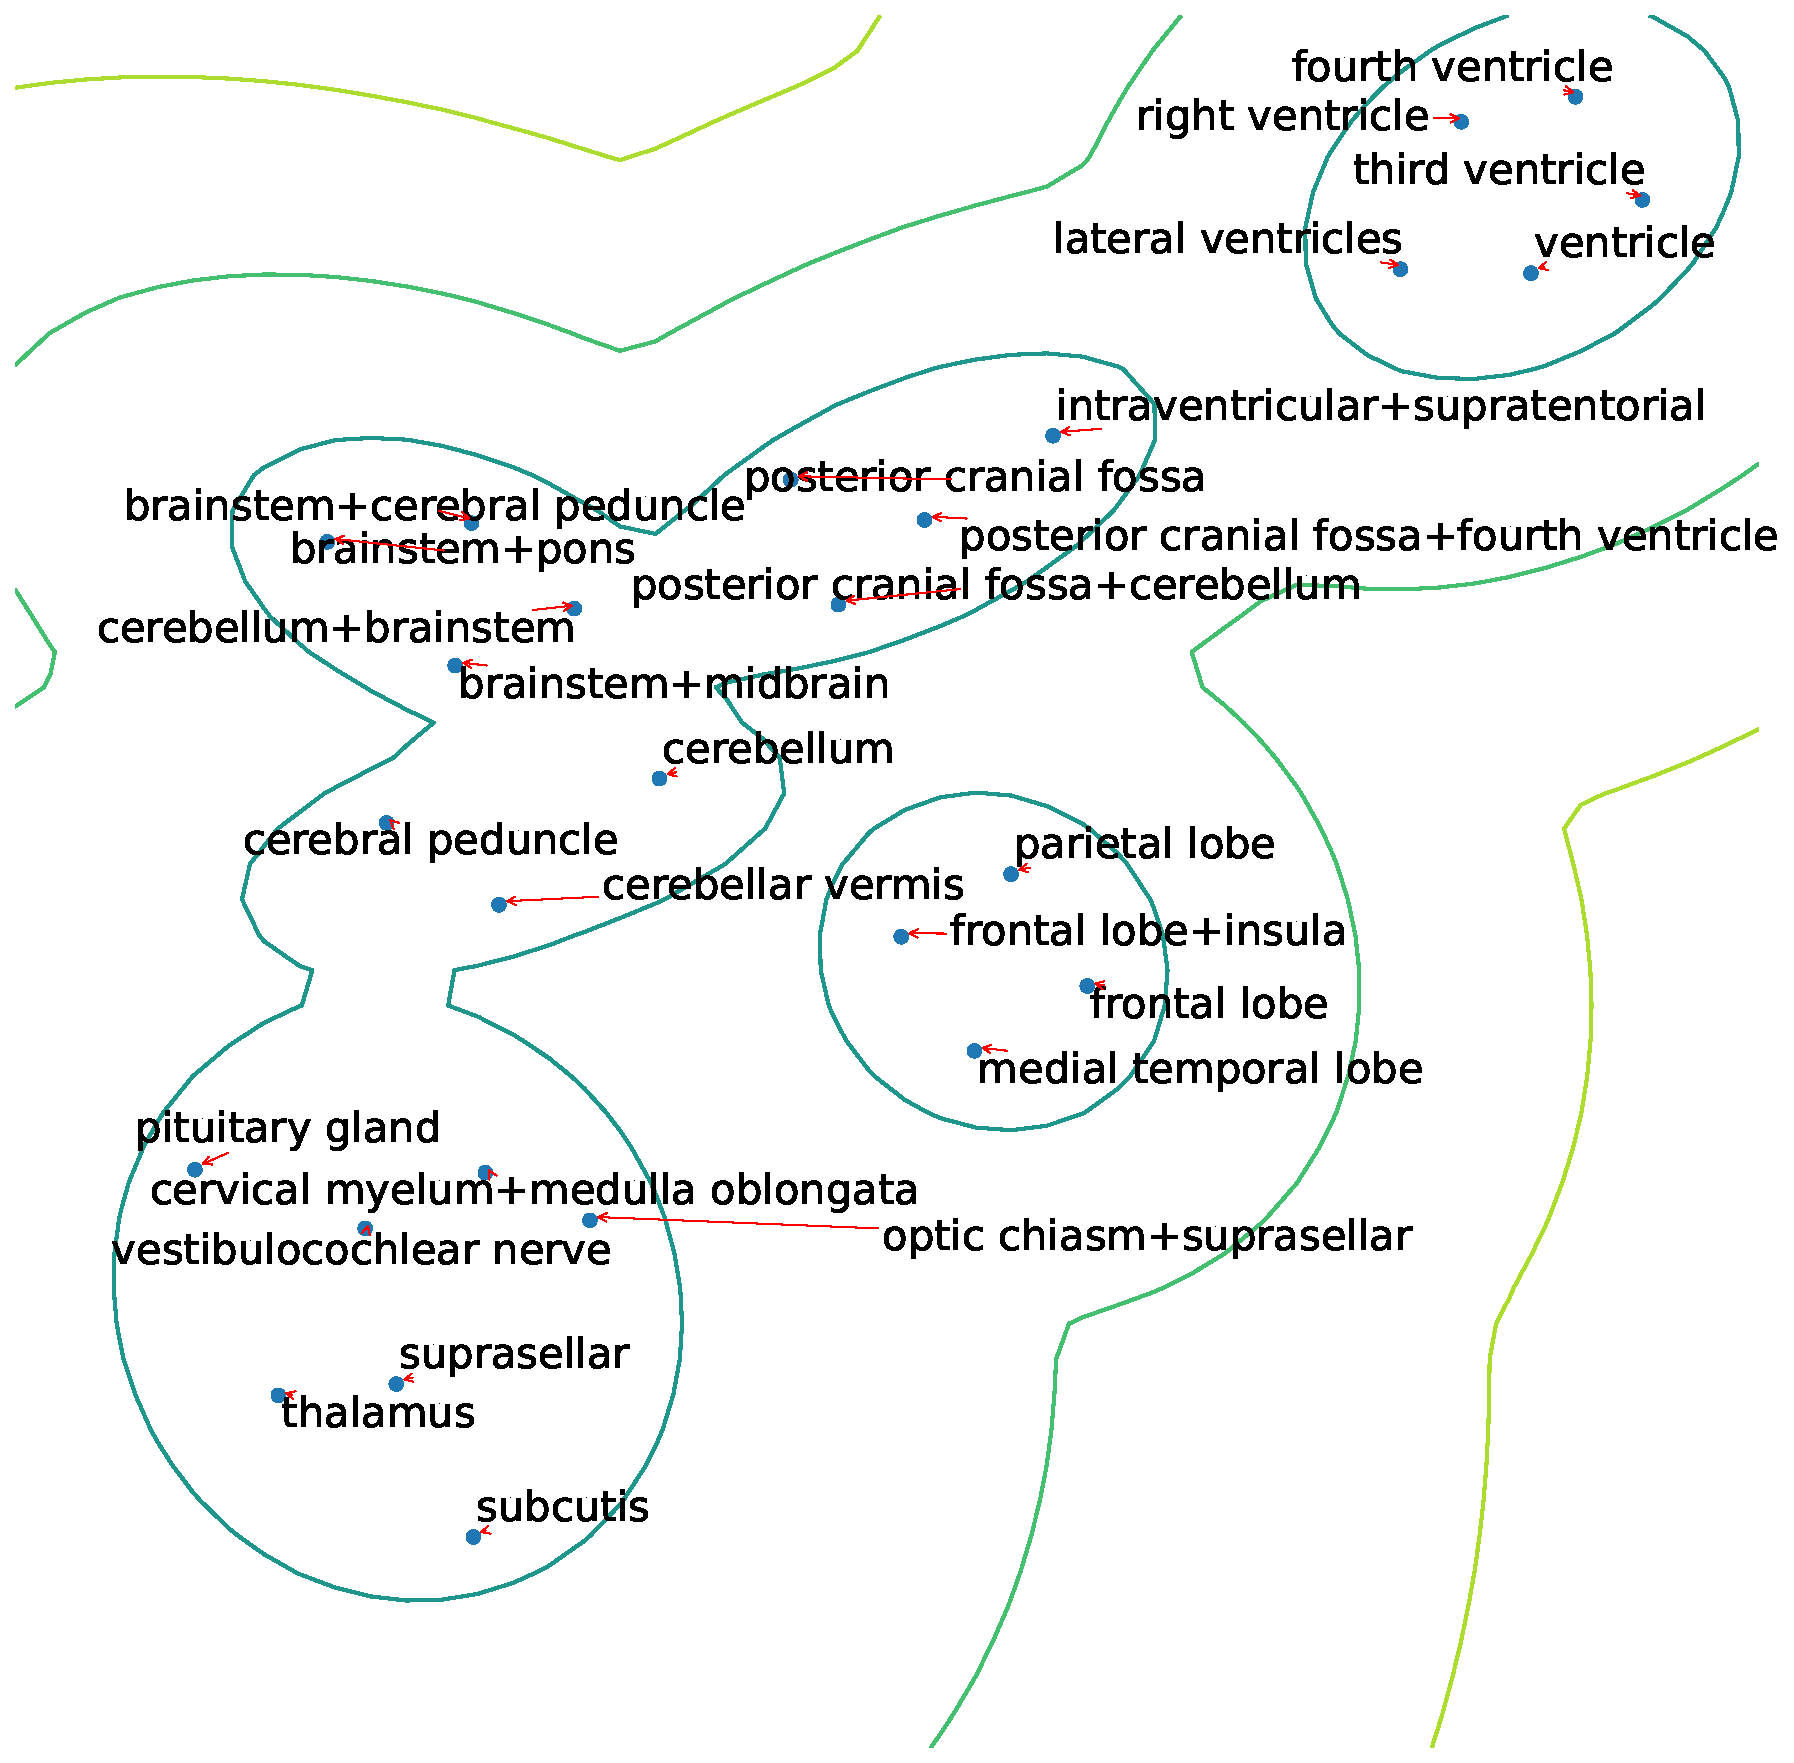
\includegraphics[width=\linewidth]{pediatric-brain-tumours/images/tsne-cc.pdf}
    \caption[T-SNE projections of location embeddings]{
        T-SNE projections (perplexity $= 8$, $10^4$ iterations) of location embeddings.
        Texts are connected to points with arrows.
        A contour plot of a six-component Gaussian mixture model to show groups of text embeddings.
    }
    \label{fig:tsne-cc}
\end{figure}
